\chapter{Jogos com agentes hiper-racionais}

Sabemos que agentes hiper-racionais podem ter como objetivo o lucro ou prejuízo para si ou qualquer outro jogador envolvido. Para quantificar essas hiper-preferências e aplicá-las no pagamento do jogador nós iremos definir a matriz de preferências $\Rc$, onde a entrada $r_{v,u}\in[-1,1]$ denota a preferência do jogador $v$ pelo jogador $u$ e $r_{v,v}\in[-1,1]$ é preferência de $v$ por si mesmo. Quando $r_{v,u}$ é positivo, o jogador $v$ busca aumentar o lucro do jogador $u$. Quando $r_{v,u}$ é negativo, o jogador $v$ busca diminuir o lucro do jogador $u$. Se $r_{v,u}$ é zero, o jogador $v$ é indiferente quanto ao lucro ou prejuízo de $u$. Além disso, vamos definir que $\Rc$ é linha estocástica em módulo, ou seja, temos que
\begin{equation}
    \sum_{u=1}^N |r_{v,u}| = 1
\end{equation}

Essa hipótese não implica em perda de generalidade, pois basta dividir as entradas de $\Rc$ por essa soma para tornar $\Rc$ linha estocástica em módulo.

Em outras palavras, o pagamento de um jogador hiper-racional é uma média ponderada entre o seu pagamento efetivo e um pagamento virtual proveniente de suas preferências, onde os pesos são as entradas da linha correspondente ao jogador na matriz $\Rc$. Com isso, dado um perfil de estratégias $\BS{X}=\{\BS{x_1},\BS{x_2},\dots,\BS{x_N}\}\in\Delta$ e as matrizes de pagamento $B_v,\forall v\in\V$, podemos definir o pagamento para agentes hiper-racionais como segue.

\begin{equation}
    \label{defPgtoHR}
    \pi^{\mathcal{H}}_v(\BS{X})=r_{v,v}\left[\BS{x_v} B_v \left(\frac{1}{N-1}\sum_{\substack{u=1\\u\neq v}}^N \BS{x_u}\right)\right] + \sum_{\substack{u=1\\u\neq v}}^N r_{v,u} \left(\BS{x_u} B_u \BS{x_v}\right)
\end{equation}

Temos agora um novo termo sendo somado na nossa função de pagamento, é o pagamento de $u$ no jogo clássico entre $u$ e $v$. Dizemos que esse termo é o pagamento de $u$ percebido por $v$ e vamos denotá-lo por

\begin{equation}
    \label{defPgtoPercebido}
    \pi^{\mathcal{H}}_{u,v}(\BS{x_u},\BS{x_v}) = \BS{x_u} B_u \BS{x_v}
\end{equation}

Note que o jogador $v$ não possui informação sobre as preferências de $u$, pois conhece apenas a estratégia mista e a matriz de pagamentos de $u$. Essa assimetria de informação é importante e suas consequências serão discutidas na seção a seguir. 

Definiremos agora o hiper-equilíbrio, que usa o pagamento $\eqref{defPgtoHR}$. Esse equilíbrio é análogo ao equilíbrio de Nash, definido em \ref{DefEqNashClassico}, porém usa o pagamento hiper-racional e tem as hiper-preferências do jogador imbuída na sua formulação. Essa distinção permite analisar separadamente os novos equilíbrios introduzidos pelas hiper-preferências dos jogadores \cite{askari2019behavioral}.

\begin{definition}
    \label{defHiperEq}
    Dado um perfil de estratégias $\BS{X^*}=(\BS{x}^*_{1},\BS{x}^*_{2},\dots,\BS{x}^*_{N})\in\Delta$ e uma matriz de preferências $\Rc$, dizemos que $\BS{X^*}$ é um hiper-equilíbrio se
    \begin{equation*}
        \pi^{\mathcal{H}}_v(\BS{x}^*_v,\BS{X}^*_{-i})\geq \pi^{\mathcal{H}}_v(\BS{x}_v,\BS{X}^*_{-i})
    \end{equation*}
    para todo $\BS{x}_v\in\Delta_{M_i}$. Se a desigualdade for estrita, dizemos que $\boldsymbol{X^*}$ é um hiper-equilíbrio estrito.
\end{definition}

%\begin{definition}[\citeauthor{askari2019behavioral}, 2019]
%    Um perfil de estratégias $\BS{X^*}$ é um hiper-equilíbrio se, para todo jogador $v\in\V$ e todo $x_v\in\Delta_M$, temos
%    \begin{equation}
%        \pi^{\mathcal{H}}_{u,v}(\BS{x^*_u},\BS{x^*_v}) \geq \pi^{\mathcal{H}}_{u,v}(\BS{x^*_u},\BS{x_v})
%    \end{equation}
%    para todo jogador $u\in\V,u\neq v$ tal que $r_{v,u}>0$ e
%    \begin{equation}
%        \pi^{\mathcal{H}}_{u,v}(\BS{x^*_u},\BS{x^*_v}) \leq \pi^{\mathcal{H}}_{u,v}(\BS{x^*_u},\BS{x_v})
%    \end{equation}
%    para todo jogador $u\in\V,u\neq v$ tal que $r_{v,u}<0$.
%\end{definition}
%Em outras palavras, um hiper-equilíbrio é um estado no qual o jogador não consegue alterar unilateralmente sua estratégia para aumentar ou diminuir o pagamento dos jogadores presentes em suas preferências. Nem todo jogo hiper-racional possui um hiper-equilíbrio e nem todo hiper-equilíbrio é também um equilíbrio de Nash. Veremos mais sobre isso com exemplos nos próximos capítulos.

Na próxima seção iremos analisar um jogo que possui um hiper-equilíbrio diferente do equilíbrio de Nash esperado por um jogador racional, mostrando na prática o motivo de haver essa separação nas definições.

% -- % -- % -- %

\section{Assimetria de informação no jogo hiper-racional}

Num primeiro momento, pode-se pensar que as preferências sociais podem ser descritas através de mudanças na matriz de pagamentos do jogador, porém o exemplo a seguir mostra que isso não é possível, pois um jogador não possui informação sobre as preferências dos demais. Considere um jogo com dois jogadores hiper-racionais, $v_1$ e $v_2$, com a matriz de pagamentos abaixo.
\begin{table}[h]
\begin{center}
    \begin{tabular}{ccccc}
        & & \multicolumn{3}{c}{$v_2$} \\
        & & $X$ & $Y$ & $Z$ \\ \cline{3-5} 
        \multirow{3}{*}{$v_1$} & \multicolumn{1}{c|}{$A$} & \multicolumn{1}{l|}{$(1,3)$} & \multicolumn{1}{l|}{$(2,4)$} & \multicolumn{1}{l|}{$(0,6)$} \\ \cline{3-5} 
        & \multicolumn{1}{c|}{$B$} & \multicolumn{1}{l|}{$(2,2)$}  & \multicolumn{1}{l|}{$(2,2)$} & \multicolumn{1}{l|}{$(1,1)$}  \\ \cline{3-5} 
        & \multicolumn{1}{l|}{$C$} & \multicolumn{1}{l|}{$(1,1)$}  & \multicolumn{1}{l|}{$(1,1)$} & \multicolumn{1}{l|}{$(0,2)$} \\ \cline{3-5} 
    \end{tabular}
    \caption{Matriz de pagamentos do jogo exemplo.}
    \label{JogoHRassimetrico}
\end{center}
\end{table}

O jogador $v_1$ é altruísta, ou seja, ele se importa com o pagamento do seu adversário, mesmo que resulte em um pagamento efetivo menor para si próprio, porém $v_2$ age como um jogador racional clássico, se importando apenas com seu pagamento. A matriz de preferências é como segue.
\begin{equation}
    \label{matrizPrefAssimetrico}
    \mathcal{R}=
    \begin{bmatrix}
        \frac{1}{2} & \frac{1}{2}\\ 
        0 & 1 
    \end{bmatrix}
\end{equation}

Assim, enquanto $v_2$ joga usando a matriz \eqref{JogoHRassimetrico}, $v_1$ joga usando uma matriz de pagamentos virtual que leva em consideração suas preferências. O pagamento virtual de $v_1$ é dado pela matriz abaixo, onde seu pagamento foi calculado de acordo com a equação \eqref{defPgtoHR}.

\begin{table}[h]
\begin{center}
    \begin{tabular}{ccccc}
        & & \multicolumn{3}{c}{$v_2$} \\
        & & $X$ & $Y$ & $Z$ \\ \cline{3-5} 
        \multirow{3}{*}{$v_1$} & \multicolumn{1}{c|}{$A$} & \multicolumn{1}{l|}{$(2,3)$} & \multicolumn{1}{l|}{$(3,4)$} & \multicolumn{1}{l|}{$(3,6)$} \\ \cline{3-5} 
        & \multicolumn{1}{c|}{$B$} & \multicolumn{1}{l|}{$(2,2)$}  & \multicolumn{1}{l|}{$(2,2)$} & \multicolumn{1}{l|}{$(1,1)$}  \\ \cline{3-5} 
        & \multicolumn{1}{l|}{$C$} & \multicolumn{1}{l|}{$(1,1)$}  & \multicolumn{1}{l|}{$(1,1)$} & \multicolumn{1}{l|}{$(1,2)$} \\ \cline{3-5} 
    \end{tabular}
    \caption{Matriz de pagamentos virtual de $v_1$.}
    \label{PagVirtualV1}
\end{center}
\end{table}

Do ponto de vista de $v_2$, podemos ver que a estratégia $B$, de $v_1$, domina fracamente todas as demais estratégias e, portanto, $v_2$ terá de decidir entre as estratégias $X$ e $Y$, pois são as que lhe dão o maior retorno contra $B$.

\begin{table}[h]
\begin{center}
    \begin{tabular}{cccc}
        & & \multicolumn{2}{c}{$v_2$} \\
        & & $X$ & $Y$ \\ \cline{3-4} 
        $v_1$ & \multicolumn{1}{c|}{$B$} & \multicolumn{1}{l|}{$(2,2)$}  & \multicolumn{1}{l|}{$(2,2)$}  \\ \cline{3-4} 
    \end{tabular}
    \caption{Matriz após a remoção das estratégias dominadas.}
\end{center}
\end{table}

Finalmente, apesar de ambas opções resultarem no mesmo pagamento, $v_2$ irá jogar $Y$, pois possui um melhor pagamento esperado contra $A$ ou $C$. Do ponto de vista de $v_1$, a estratégia $A$ domina fracamente todas as demais e, portanto, será a sua escolha. Assim, o hiper-equilíbrio desse jogo é dado pelo perfil $(A,Y)$, com pagamento efetivo $(2,4)$, enquanto os equilíbrios de Nash, esperados por $v_2$, são dados por $(B,Y)$ e $(B,X)$, com pagamento efetivo $(2,2)$.

Além disso, se as preferências pudessem ser simplesmente traduzidas na matriz de pagamento o equilíbrio seria dado pelo perfil $(A,Z)$, pois $v_2$ iria explorar o altruísmo de $v_1$ para obter um pagamento maior para si mesmo. Esse comportamento só acontece por conta da assimetria de informação entre os jogadores. Cada jogador possui um pagamento virtual próprio que influencia suas decisões e, como vimos no exemplo acima, muda o resultado do jogo. Porém, em um jogo iterado, $v_2$ seria capaz de, eventualmente, descobrir e explorar o altruísmo de $v_1$. Esse comportamento é esperado de um jogador racional, que busca o melhor pagamento para si, mas ainda assim o resultado seria diferente dos equilíbrios de Nash do jogo.

% -- % -- % -- %

\section{Dilema do prisioneiro hiper-racional}

No início deste trabalho nós introduzimos o Dilema do Prisioneiro com matriz de pagamentos \ref{mpdp} e vimos que o perfil de estratégias $\{\textit{delação},\textit{delação}\}$ era o único equilíbrio de Nash do jogo. Agora vamos considerar o mesmo jogo, com a mesma matriz de pagamentos, porém com $v_1$ e $v_2$ como jogadores hiper-racionais.

Como nesse jogo temos apenas dois jogadores e duas estratégias podemos denotar a matriz de preferências dos jogadores como

\begin{equation}
    \label{matrizPrefPD}
    \mathcal{R}=
    \begin{bmatrix}
        r_1 & 1-r_1\\ 
        1-r_2 & r_2 
    \end{bmatrix}
\end{equation}
onde $r_1,r_2\in[0,1]$ denotam a preferência do jogador por si mesmo. Vamos desconsiderar valores negativos para as preferências nesse jogo, pois o pagamento virtual da estratégia $\textit{delação}$ aumenta quando um jogador tem preferência negativa pelo outro, somente reforçando a dominância do jogo clássico, e o pagamento virtual da estratégia $\textit{silêncio}$ se torna dominante quando um jogador tem preferência negativa por si mesmo. 

Denotaremos a probabilidade do jogador $i=1,2$ usar a estratégia $\textit{silêncio}$ por $x_{i,s}$ e a estratégia $\textit{delação}$ por $x_{i,d}=(1-x_{i,s})$. Assim, sendo $j$ o adversário de $i$, a equação de replicação para esse jogo é dada por
\begin{equation}
\begin{split}
    \label{eqRepPDHREx}
    \dot{x}_{i,s}&= \!\begin{multlined}[t]
    x_{i,s}(1-x_{i,s})\left\{x_{j,s}\left[r_i(-2)+(1-r_i)(5)\right]\right.\\
    + \left. (1-x_{j,s})\left[r_i(-2)+(1-r_i)(5)\right] \right\}
    \end{multlined} \\
    &= x_{i,s}(1-x_{i,s})\left[ r_i(-2)+(1-r_i)(5) \right] \\
    &= x_{i,s}(1-x_{i,s})\left[ 5-7r_i \right]
\end{split}
\end{equation}

Note que a variação nas probabilidades de $i$ dependem somente de suas hiper-preferências, sendo completamente independente do perfil de estratégias do seu adversário. De fato, para valores de $r_i$ maiores que $\frac{5}{7}$ o jogador $i$ irá, eventualmente, sempre escolher $\textit{delação}$, para valores menores que $\frac{5}{7}$ irá sempre escolher $\textit{silêncio}$ e para valores iguais à $\frac{5}{7}$ o estado inicial de $i$ será seu estado de hiper-equilíbrio. Esse comportamento pode ser observado na figura \ref{fig:pd-neg-payoff}.

\begin{figure}[h]
    \caption{Probabilidade do jogador usar \textit{silêncio}, onde a condição inicial é 0.5 para todas estratégias para ambos jogadores.}
    \centerline{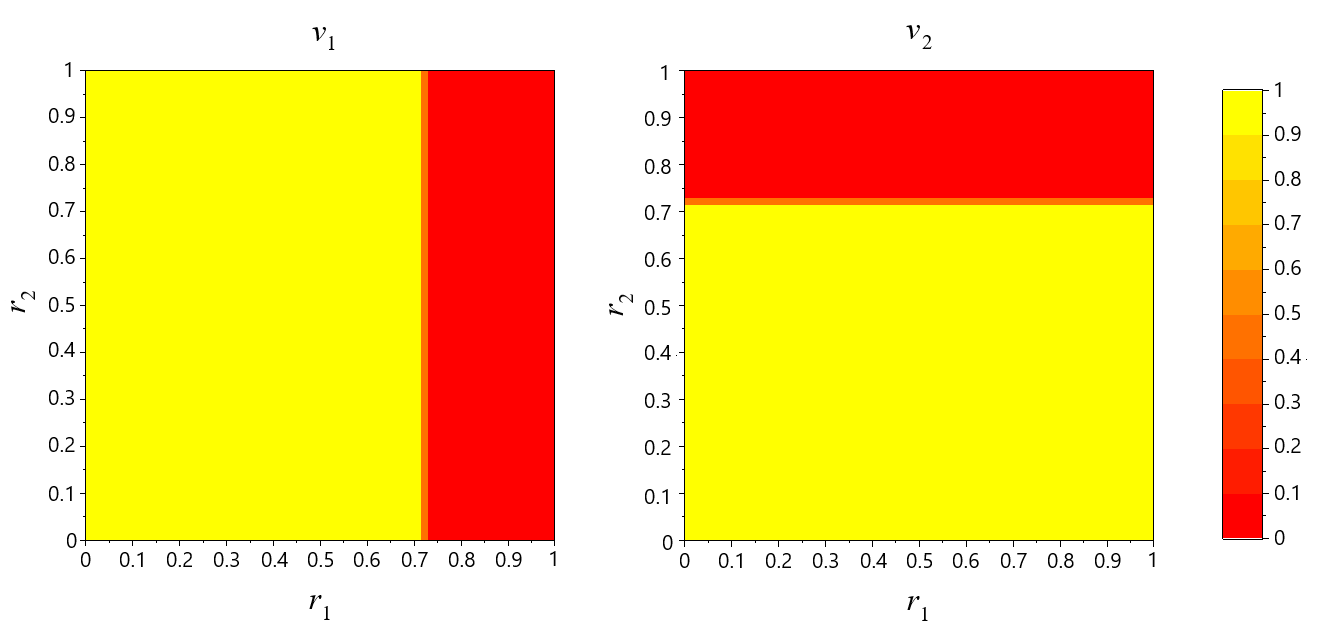
\includegraphics[scale=0.43]{./img/PD-neg-payoff.png}}
    \label{fig:pd-neg-payoff}
\end{figure}

Nos interessa saber se esse comportamento é geral ou uma exceção e, por isso, vamos usar um definição mais geral para o pagamento do dilema do prisioneiro, dada por
\begin{equation}
    \label{payoffGeralPD}
    B=
    \begin{bmatrix}
        R & S\\ 
        T & P 
    \end{bmatrix}
\end{equation}
onde $R$ é a recompensa pela cooperação entre os jogadores, $T$ é a tentação para trair, $P$ é a punição pela traição mútua e $S$ é o pagamento do ingênuo, que foi traído. Para que esses valores representem um dilema do prisioneiro eles devem respeitar a seguinte restrição.

\begin{equation}
    T>R>P>S
\end{equation}

Assim, a equação de replicação para um dilema do prisioneiro geral é dada por

\begin{equation}
\begin{split}
    \label{eqRepPDGeral}
    \dot{x}_{i,s}&= \!\begin{multlined}[t]
        x_{i,s}(1-x_{i,s})\left\{x_{j,s}\left[r_i(R-T)+(1-r_i)(R-S) \right] \right.\\
        + \left. (1-x_{j,s})\left[r_i(S-P)+(1-r_i)(T-P)\right] \right\}
    \end{multlined} \\
    &= \!\begin{multlined}[t]
    x_{i,s}(1-x_{i,s})\left\{r_i \left[x_{j,s}(R-T)+(1-x_{j,s})(S-P) \right] \right. \\
    + \left. (1-r_i)\left[ x_{j,s}(R-S) + (1-x_{j,s})(T-P)\right] \right\}
    \end{multlined}
\end{split}
\end{equation}

Um jogador não tem incentivos de mudar sua estratégia quando $\dot{x}_{i,s}=0$. Portanto, vamos assumir que $\dot{x}_{i,s}=0$ para algum perfil de estratégias $\BS{X}$ e, assim, a equação $\eqref{eqRepPDGeral}$ se torna
\begin{equation}
    0 = \!\begin{multlined}[t]
        r_i \left[x_{j,s}(R-T)+(1-x_{j,s})(S-P) \right] \\
    + (1-r_i)\left[ x_{j,s}(R-S) + (1-x_{j,s})(T-P)\right]
    \end{multlined}
\end{equation}
que podemos simplificar da para obtermos
\begin{equation}
    0 = r_i(S-T) + x_{j,s}(R-S) + (1-x_{j,s})(T-P)
\end{equation}
e, por fim, isolamos $r_i$ para obter
\begin{equation}
    \label{rSela}
    r_i=\frac{x_{j,s}(T+S-P-R)+P-T}{S-T}
\end{equation}

Com isso, se a igualdade 
\begin{equation}
    \label{condicaoIndependencia}
    T+S-P-R = 0
\end{equation}
for satisfeita, basta que tenhamos
\begin{equation}
    r_i=\frac{P-T}{S-T}
\end{equation}
para que $\dot{x}_{i,s}=0$ para todo $t>0$, fazendo com que a condição inicial de $i$ seja um hiper-equilíbrio. Note que a igualdade $\eqref{condicaoIndependencia}$ é, de fato, satisfeita para os pagamentos de \ref{mpdp}, $R=-2,S=-7,T=0,P=-5$. Além disso, a igualdade $\eqref{rSela}$ nos dá uma forma de encontrar o ponto de sela, onde qualquer variação em $r_i$, para mais ou para menos, vai alterar o resultado do jogo. Também podemos ver uma ligação entre $r_i$ e $x_{j,s}$, que iremos avaliar agora.

Podemos alterar a matriz \ref{mpdp} para que haja uma dependência diretamente proporcional entre $r_i$ e $x_{j,s}$, basta tomar $R=-1$, assim a equação $\eqref{rSela}$ se torna
\begin{equation}
    r_i=\frac{5+x_{j,s}}{7}
\end{equation}

Como $x_{j,s}\in[0,1]$, para valores de $r_i$ no intervalo $[\frac{5}{7},\frac{6}{7}]$ a distribuição de estratégias do jogador $i$ depende diretamente da distribuição de $j$. Assim, como a matriz de pagamentos é igual para ambos jogadores, esse intervalo de dependência é igual para os dois jogadores e a solução dentro do quadrado $[\frac{5}{7},\frac{6}{7}]\times[\frac{5}{7},\frac{6}{7}]$ dependerá da distribuição de estratégias de ambos. Esse comportamento pode ser observado na figura \ref{fig:pd-neg-payoff-dependant}, onde o ponto de sela da solução se encontra na diagonal do quadrado $[\frac{5}{7},\frac{6}{7}]\times[\frac{5}{7},\frac{6}{7}]$. Também é interessante notar que a estratégia $\textit{silêncio}$ é predominante no nosso gráfico, pois $\textit{delação}$ só é vantajoso para de $r_i$ bem próximos de $1$.

\begin{figure}[h]
    \caption{Probabilidade do jogador usar \textit{silêncio} ao tomar $R=-1$ no pagamento dado por \ref{mpdp}, onde a condição inicial é 0.5 para todas estratégias para ambos jogadores.}
    \centerline{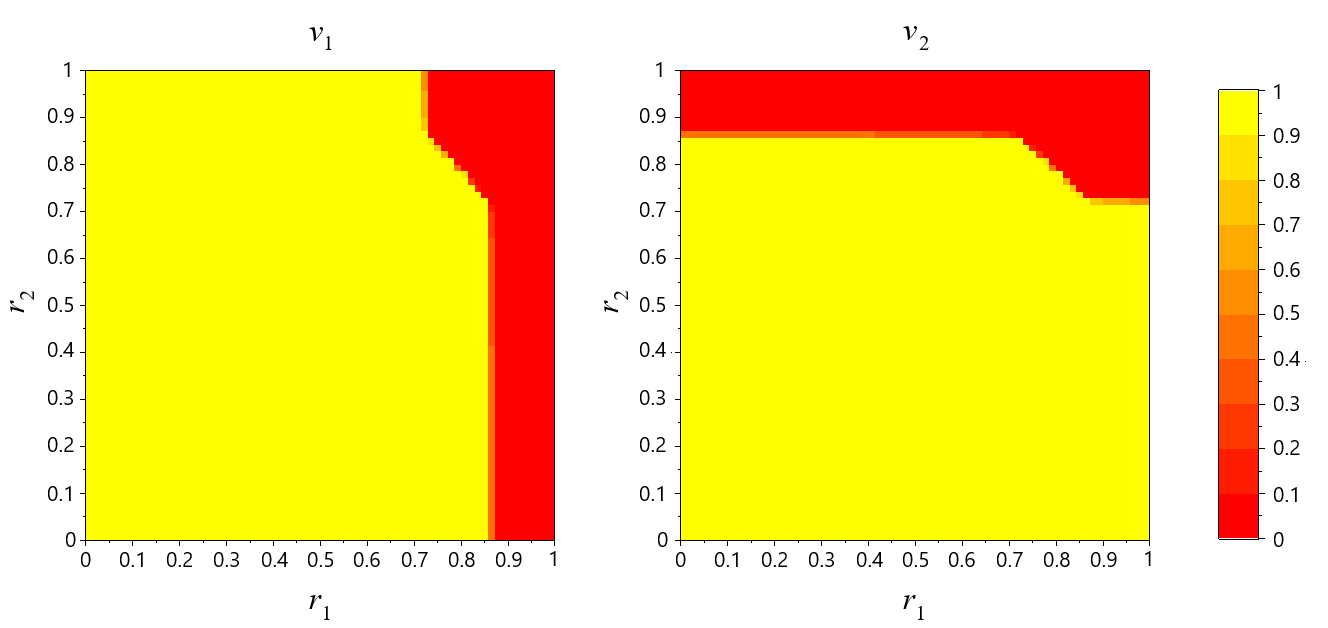
\includegraphics[scale=0.43]{./img/PD-neg-payoff-dependant.png}}
    \label{fig:pd-neg-payoff-dependant}
\end{figure}

Da mesma maneira, podemos novamente usar o pagamento definido em \ref{mpdp} e tomar $S=-6$ para que haja uma dependência inversamente proporcional entre $r_i$ e $x_{j,s}$, assim a equação $\eqref{rSela}$ se torna
\begin{equation}
    r_i=\frac{5-x_{j,s}}{6}
\end{equation}

Agora temos $[\frac{4}{6},\frac{5}{6}]$ como nosso intervalo de dependência que, novamente, é igual para ambos jogadores. Agora o ponto de sela estará na diagonal do quadrado $[\frac{4}{6},\frac{5}{6}]\times[\frac{4}{6},\frac{5}{6}]$ e, apesar de ainda não ser predominante, a faixa na qual $\textit{delação}$ se torna mais vantajosa aumentou consideravelmente.

\begin{figure}[h]
    \caption{Probabilidade do jogador usar \textit{silêncio} ao tomar $S=-6$ no pagamento dado por \ref{mpdp}, onde a condição inicial é 0.5 para todas estratégias para ambos jogadores.}
    \centerline{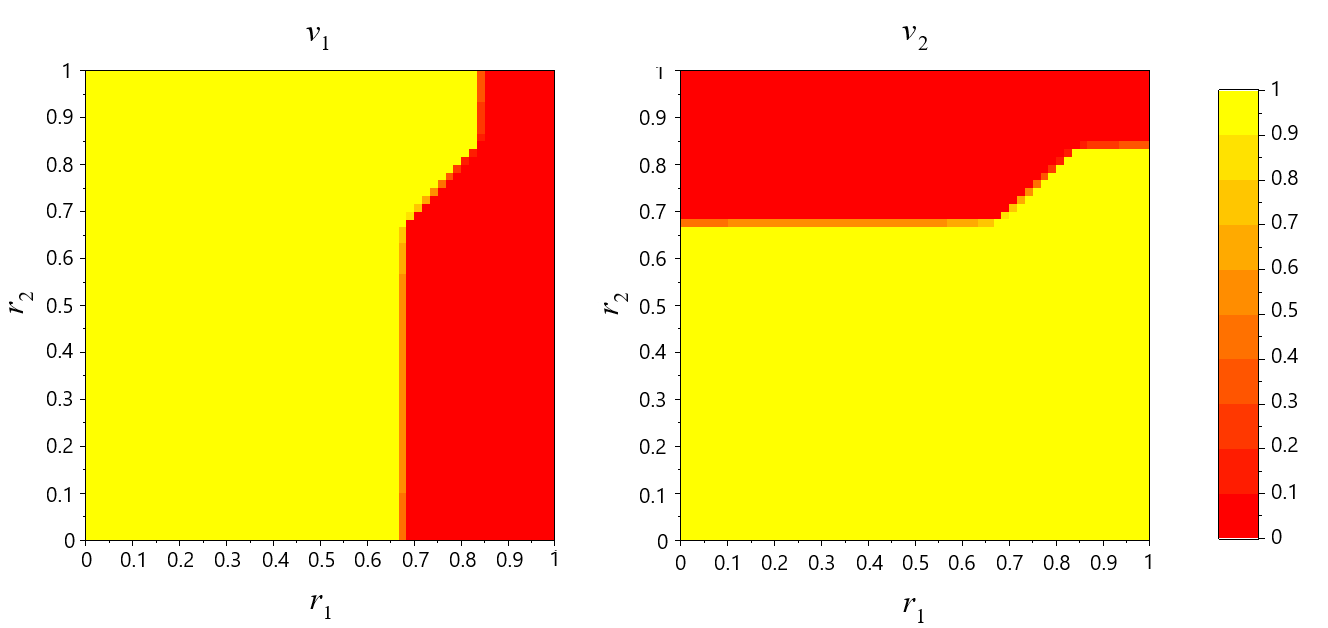
\includegraphics[scale=0.43]{./img/PD-neg-payoff-inverse-dep.png}}
    \label{fig:pd-neg-payoff-inverse-dep}
\end{figure}

A hiper-racionalidade dos jogadores envolvidos faz com que a estratégia $\textit{silêncio}$ se torne, em geral, mais atraente para o jogador mesmo que a condição inicial não esteja muito próxima de $\textit{silêncio}$, enquanto jogadores racionais, mesmo em redes, tendem a preferir $\textit{delação}$ se houver algum vizinho delator \cite{madeo2015}.

Na figura \ref{fig:sobreposicao} temos a sobreposição dos gráficos dos dois jogadores para cada pagamento discutido acima. Assim, podemos ver o resultado do jogo em cada uma das faixas de $r_i$ analisadas anteriormente, explicitando a predominância da estratégia $\textit{silêncio}$ e o fato de que, em muitos casos, um jogador recebe o pagamento do ingênuo $S$, mesmo podendo aumentar seu pagamento efetivo trocando sua estratégia para $\textit{delação}$.

\begin{figure}[h]
    \caption{Sobreposição dos resultados do Dilema do Prisioneiro para cada pagamento apresentado anteriormente. Nos parênteses temos, respectivamente, o resultado do jogador $v_1$ e $v_2$, com $s$ para $\textit{silêncio}$ e $d$ para $\textit{delação}$.}
    \centerline{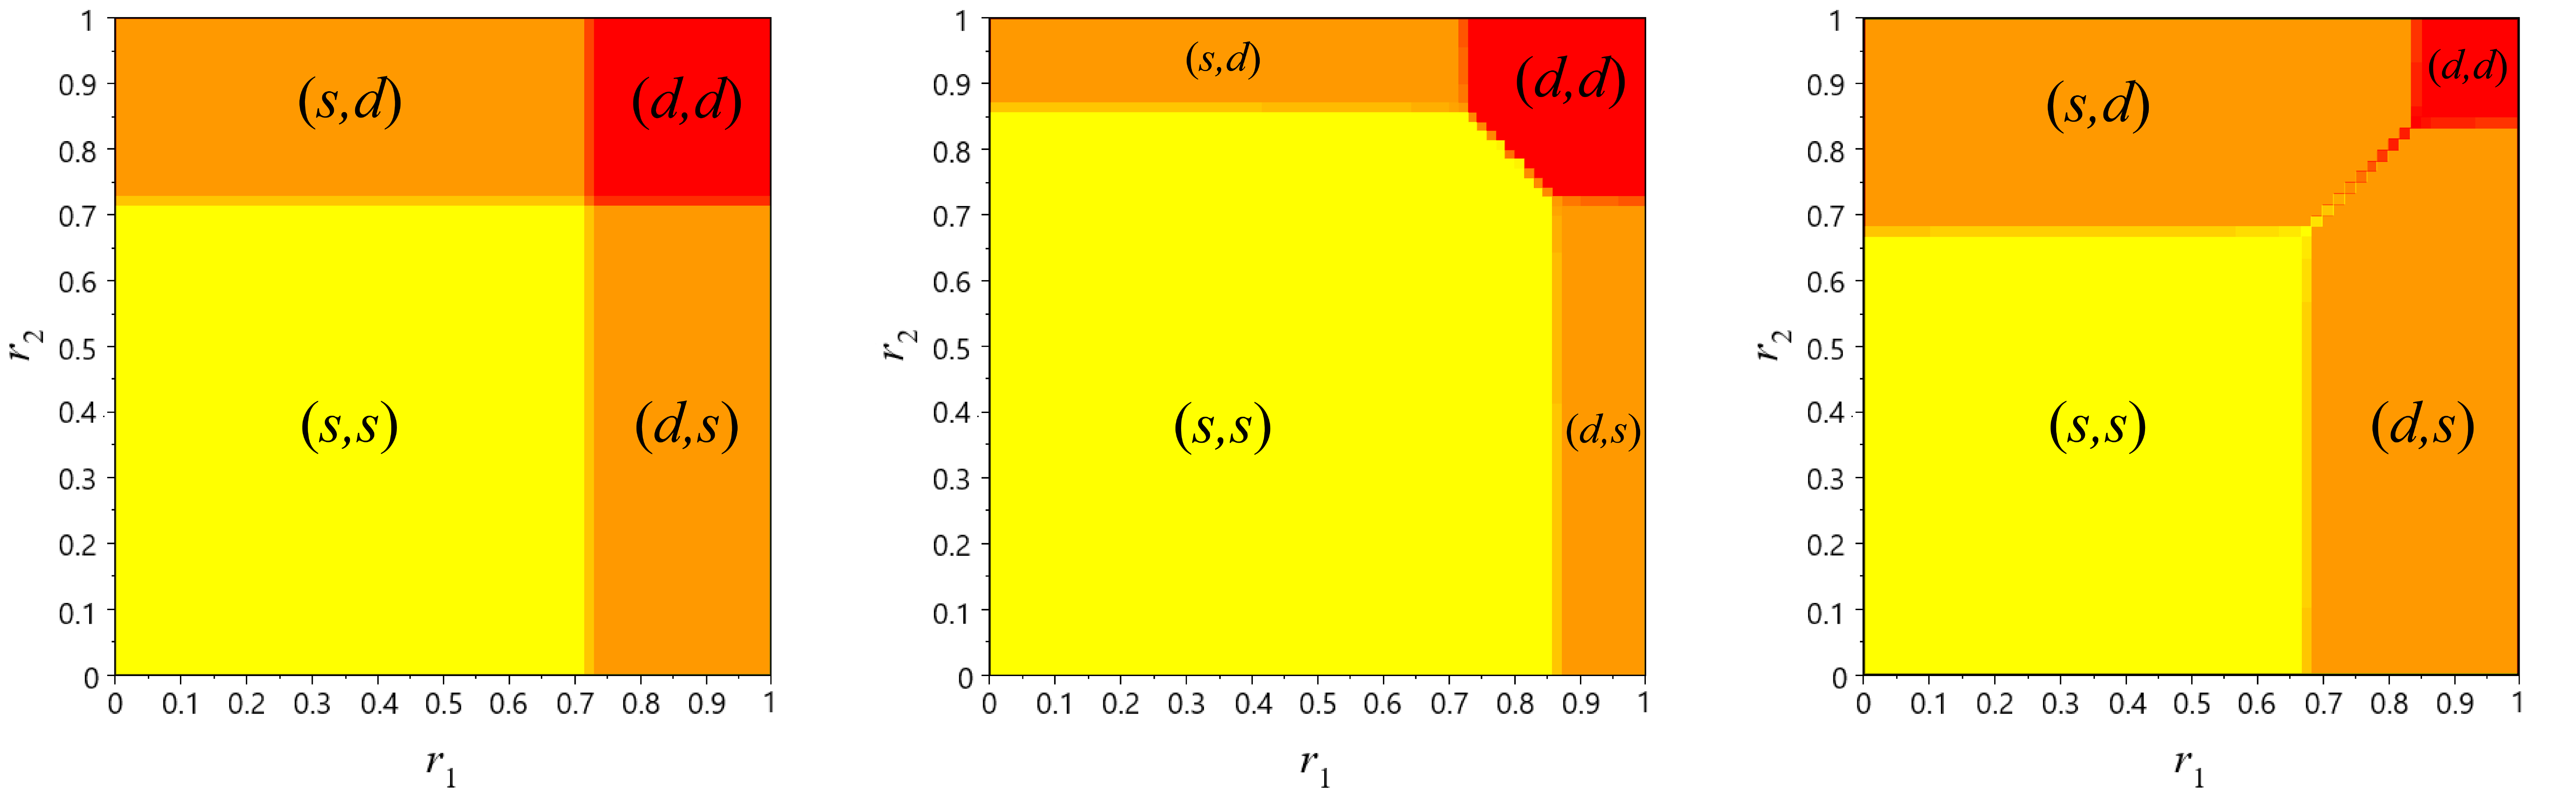
\includegraphics[scale=0.0775]{./img/sobreposicao.png}}
    \label{fig:sobreposicao}
\end{figure}

Essa sobreposição nada mais é do que a soma das probabilidades de $v_1$ e $v_2$ dividida por $2$ exibida na mesma escala das demais figuras desta seção. Assim, as faixas de transição em $\frac{5}{7}$ e nas diagonais dos quadrados $[\frac{5}{7},\frac{6}{7}]\times[\frac{5}{7},\frac{6}{7}]$ e $[\frac{4}{6},\frac{5}{6}]\times[\frac{4}{6},\frac{5}{6}]$ exibem a cor que representa essa média das probabilidades.